\section{欧氏公理体系}
\subsection{几何元素}
\begin{definition}\label{definition:欧氏几何.几何元素.基本几何元素}
在平面几何中,有两种基本研究对象:
\begin{enumerate}
	\item \DefineConcept{点}(我们常用大写拉丁字母\(A,B,C,\dotsc\)表示);
	\item \DefineConcept{直线}(我们常用小写拉丁字母\(a,b,c,\dotsc\)表示).
\end{enumerate}
在空间几何中,除了上述两种以外,还多了一种研究对象:
\begin{enumerate}
\setcounter{enumi}{2}
	\item \DefineConcept{平面}(我们常用小写希腊字母\(\alpha,\beta,\gamma,\dotsc\)表示).
\end{enumerate}
点和直线统称为“平面几何的\emph{元素}”;
点、直线和平面统称为“空间几何的\emph{元素}”.
\end{definition}

我们设想,点、直线、平面这三类几何元素之间总是存在某种关系.
根据这些关系,我们提出以下五组命题,并认定它们恒为真,特别地称它们为“公理(axiom)”.

\subsection{第一组公理:关联公理}
本组公理是在前面提到的点、直线和平面这三类几何元素之间建立联系,其条文如下.
\begin{axiom}[关联公理]\label{axiom:欧氏几何.关联公理}
点、直线和平面这三类几何元素存在如下的关系:
\begin{enumerate}
\item 对于两点\footnote{%
在本章中,当提到“两点”“两条直线”等时,都是指两个相异的几何元素.%
}\(A\)和\(B\),
恒有一直线\(l\),
它同\(A\)和\(B\)这两点的每一点都相关\footnote{%
同一种关系可能存在多种说法,
例如“直线\(l\)同\(A\)和\(B\)这两点的每一点都相关”
可以说成是“直线\(l\)通过点\(A\)、点\(B\)”
或“直线\(l\)连结点\(A\)和点\(B\)”,
而“点\(A\)与直线\(l\)相关”可以说成是“点\(A\)在直线\(l\)上”
“点\(A\)是直线\(l\)(上)的一点”或“直线\(l\)含有点\(A\)”.%
“点\(P\)既在直线\(a\)上,
又在直线\(b\)上”可以说成是“点\(P\)是直线\(a\)和直线\(b\)的\DefineConcept{交点}或\DefineConcept{公共点}”
或“直线\(a\)、\(b\)相交于点\(P\)”.
}.

\item 对于两点\(A\)和\(B\),
至多有一直线\footnote{%
除了可以用某个小写拉丁字母表示直线以外,与点\(A\)、\(B\)相关的直线还可以记作\(AB\).%
},它同\(A\)和\(B\)这两点的每一点都相关.

\item 一直线上恒至少有两点;至少有三点不在同一直线上.

\item 对于不在同一直线上的任意三点\(A\)、\(B\)和\(C\),恒有一平面\(\gamma\),它同\(A\)、\(B\)和\(C\)这三点的每一点相关;对于任一平面,恒有一点同这平面相关\footnote{%
“点\(A\)与平面\(\gamma\)相关”可以说成是“点\(A\)在\(\gamma\)上”或“点\(A\)是\(\gamma\)的点”.%
}.

\item 对于不在同一直线上的三点\(A\)、\(B\)和\(C\),至多有一平面\footnote{%
除了可以用某个小写希腊字母表示平面以外,由点\(A\)、\(B\)和\(C\)确定的平面还可以记作\(ABC\).%
},它同\(A\)、\(B\)和\(C\)这三点的每一点相关.

\item 若一直线\(l\)的两点\(A\)和\(B\)在一平面\(\gamma\)上,则\(l\)的每一点都在平面\(\gamma\)上\footnote{%
或者说“直线\(l\)在平面\(\gamma\)上”.%
}.

\item 若两平面\(\alpha\)和\(\beta\)有一个公共点\(A\),则它们至少还有一个(与\(A\)相异的)公共点\(B\)\footnote{%
这表明空间的维数不大于3.%
}.

\item 至少有四点不在同一平面上\footnote{%
这表明空间的维数不小于3.%
}.
\end{enumerate}
\end{axiom}
\cref{axiom:欧氏几何.关联公理}
的前3个命题可以统称为{\bf 平面公理},
后5个命题可以统称为{\bf 空间公理}.

依据\cref{axiom:欧氏几何.关联公理} 可以推证出以下两条定理.
\begin{theorem}\label{theorem:欧氏几何.定理1}
一平面上的两直线或有一公共点,或无公共点;
两平面或无公共点,或有一公共直线;
两平面无公共直线时无公共点;
一平面和不在其上的一直线或无公共点,或有一公共点.
\end{theorem}

\begin{theorem}\label{theorem:欧氏几何.定理2}
过一直线和不在这直线上的一点,或过有公共点的两条不同直线,恒有一个而且只有一个平面.
\end{theorem}

\subsection{第二组公理:顺序公理}
本组公理规定了“介于”(或“在……之间”)这个概念.
根据这个概念,直线上的、平面上的和空间中的点才有顺序可言.
\begin{axiom}[顺序公理I]\label{axiom:欧氏几何.顺序公理1}
在一直线上的点有一定的相互关系.
我们特别用“介于”(或“在……之间”)来描述它.
\begin{enumerate}
	\item 若一点\(B\)在一点\(A\)和一点\(C\)之间
	(如\cref{figure:欧氏几何.直线上点的顺序1}),
	则\(A\)、\(B\)和\(C\)是一直线上的不同的三点,
	同时\(B\)也在\(C\)和\(A\)之间.
	\begin{figure}[htb]
		\centering
		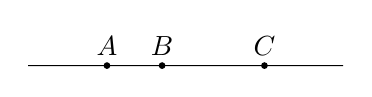
\begin{tikzpicture}
			\draw[fill=black] (0,0)--(1,0)node[above]{\(A\)}circle(1pt)
			--(1.7,0)node[above]{\(B\)}circle(1pt)
			--(3,0)node[above]{\(C\)}circle(1pt)
			--(4,0);
		\end{tikzpicture}
		\caption{直线上点的顺序}
		\label{figure:欧氏几何.直线上点的顺序1}
	\end{figure}

	\item 对于两点\(A\)和\(B\)(如\cref{figure:欧氏几何.直线上点的顺序2}),
	直线\(AB\)上恒至少有一点\(C\),使得\(B\)在\(A\)和\(C\)之间.
	\begin{figure}[htb]
		\centering
		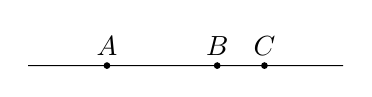
\begin{tikzpicture}
			\draw[fill=black] (0,0)--(1,0)node[above]{\(A\)}circle(1pt)
			--(2.4,0)node[above]{\(B\)}circle(1pt)
			--(3,0)node[above]{\(C\)}circle(1pt)
			--(4,0);
		\end{tikzpicture}
		\caption{直线上点的顺序}
		\label{figure:欧氏几何.直线上点的顺序2}
	\end{figure}

	\item 一直线的任意三点中,至多有一点在其他两点之间.
\end{enumerate}
\end{axiom}

在上述三条{\bf 直线顺序公理}之外,还需要一条{\bf 平面顺序公理}.

\begin{axiom}[顺序公理II]\label{axiom:欧氏几何.顺序公理2}
考虑一直线\(l\)上的两点\(A\)和\(B\).
我们把这一对点\(A\)和\(B\)确定的介于它们的点的集合叫做一条\DefineConcept{线段},记作\(AB\)(或\(BA\)).
在\(A\)和\(B\)之间的点叫做线段\(AB\)的点,或线段\(AB\)的\DefineConcept{内点};
\(A\)和\(B\)叫做线段\(AB\)的\DefineConcept{端点};
直线\(l\)上的其他点叫做线段\(AB\)的\DefineConcept{外点}.
\begin{enumerate}
	\setcounter{enumi}{3}
	\item 设\(A\)、\(B\)和\(C\)是不在同一直线上的三点,
	\(l\)是平面\(ABC\)上的一直线,
	但\(l\)不通过\(A,B,C\)这三点中的任一点
	(如\cref{figure:欧氏几何.平面上点的顺序1}),
	若直线\(l\)通过线段\(AB\)的一点,则它必定也通过线段\(AC\)或线段\(BC\)的一点.
	\begin{figure}[htb]
		\centering
		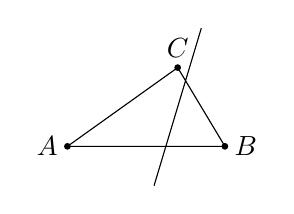
\begin{tikzpicture}
			\draw[fill=black] (-1,0)node[left]{\(A\)}circle(1pt)
			--(1,0)node[right]{\(B\)}circle(1pt)
			--(.4,1)node[above]{\(C\)}circle(1pt)--(-1,0)
			(.1,-.5)--(.7,1.5);
		\end{tikzpicture}
		\caption{平面上点的顺序}
		\label{figure:欧氏几何.平面上点的顺序1}
	\end{figure}
\end{enumerate}
\end{axiom}
直观地说,\cref{axiom:欧氏几何.顺序公理2} 说的就是:
若一直线“冲进”一个三角形的内部,它必定还要再“冲出”这个三角形.
易证:与线段\(AB\)相交的直线\(l\)不同时和\(AC,BC\)这两条线段都相交.

\subsection{关联公理和顺序公理的推论}
从\cref{axiom:欧氏几何.关联公理,axiom:欧氏几何.顺序公理1,axiom:欧氏几何.顺序公理2} 能推证下列定理.
\begin{theorem}\label{theorem:欧氏几何.定理3}
对于两点\(A\)和\(C\),直线\(AC\)上恒至少有一点\(D\),在\(A\)和\(C\)之间.
\begin{proof}
根据\cref{axiom:欧氏几何.关联公理} 第3条,直线\(AC\)外存在一点\(E\);
根据\cref{axiom:欧氏几何.顺序公理1} 第2条,直线\(AE\)上有一点\(F\),使得\(E\)在线段\(AF\)内.
根据\cref{axiom:欧氏几何.顺序公理1} 第2条、第3条,直线\(FC\)上有一点\(G\),不在线段\(FC\)内.
根据\cref{axiom:欧氏几何.顺序公理2} 第4条,直线\(EG\)必交线段\(AC\)于一点\(D\).
\end{proof}
\end{theorem}

\begin{theorem}\label{theorem:欧氏几何.定理4}
一直线上的任意三点\(A,B,C\)中,必有一点且只有一点在其他两点之间.
\begin{proof}
设\(A\)不在\(B\)和\(C\)之间,而且\(C\)不在\(A\)和\(B\)之间.
用直线连接\(B\)和直线\(AC\)外一点\(D\).
根据\cref{axiom:欧氏几何.顺序公理1} 第2条,能在直线\(BD\)上取一点\(G\),使得\(D\)在\(B\)和\(G\)之间.
对于三角形\(BCG\)和直线\(AD\)应用\cref{axiom:欧氏几何.顺序公理2} 第4条,可知直线\(AD\)通过线段\(CG\)内的一点\(E\);
同理可知直线\(CD\)通过线段\(AG\)内一点\(F\).
对于三角形\(AEG\)和直线\(CF\)应用\cref{axiom:欧氏几何.顺序公理2} 第4条,可知\(D\)在\(A\)和\(E\)之间;
再对于三角形\(AEC\)和直线\(BG\)应用\cref{axiom:欧氏几何.顺序公理2} 第4条,即证得\(B\)在\(A\)和\(C\)之间.
\end{proof}
\end{theorem}

\begin{theorem}\label{theorem:欧氏几何.定理5}
一直线上的任意四点\(A,B,C,D\),使得点\(B\)既在\(A\)和\(C\)之间,又在\(A\)和\(D\)之间;
而且点\(C\)既在\(A\)和\(D\)之间,又在\(B\)和\(D\)之间.
\end{theorem}

\begin{corollary}\label{theorem:欧氏几何.定理6}
一直线上的任意有限个点\(A,B,C,\dotsc,K\),
使得点\(B\)在\(A\)和\(C\),或和\(D\),或和\(E\),……,或和\(K\)之间;
而且点\(C\)在\(A\)(或\(B\))和\(D\),或和\(E\),……,或和\(K\)之间;以此类推.
\end{corollary}

\begin{corollary}\label{theorem:欧氏几何.定理7}
一直线上任意两点之间恒有无限多个点.
\end{corollary}

\begin{theorem}\label{theorem:欧氏几何.定理8}
一平面\(\gamma\)上的任一直线\(l\)将该平面上其余的点分为具有下述性质的两个区域:
一个区域的任一点\(A\)与另一区域的任一点\(B\)所决定的线段\(AB\)内,
必含有直线\(l\)的一点(如\cref{figure:欧氏几何.直线l分平面为两个区域});
而同一个区域的任意两点\(A\)和\(A'\)所决定的线段\(AA'\)内,不含有直线\(l\)的点.
\begin{figure}[htb]
\centering
\begin{tikzpicture}
\draw (-2,0)--(2,0)node[right]{\(l\)}
(.5,-1)node[right]{\(B\)}--(-.5,.5)node[left]{\(A\)}--(.3,1)node[right]{\(A'\)};
\end{tikzpicture}
\caption{直线\(l\)分平面为两个区域}
\label{figure:欧氏几何.直线l分平面为两个区域}
\end{figure}
\end{theorem}

\begin{definition}
我们说\(A\)和\(A'\)这两点在平面\(\gamma\)上直线\(l\)的\DefineConcept{同侧}%
(如\cref{figure:欧氏几何.直线l分平面为两个区域}),
而\(A\)和\(B\)这两点在平面\(\gamma\)上直线\(l\)的\DefineConcept{异侧}.
\end{definition}

\begin{definition}
设\(A,A',O\)和\(B\)是一直线\(l\)上的四点(如\cref{figure:欧氏几何.射线}),
而\(O\)在\(A\)和\(B\)之间,但不在\(A\)和\(A'\)之间.
我们称“\(A\)和\(A'\)这两点在\(l\)上点\(O\)的\DefineConcept{同侧}”,
而称“\(A\)和\(B\)这两点在\(l\)上点\(O\)的\DefineConcept{异侧}”.

直线\(l\)上点\(O\)的同侧的点的全体,叫做从点\(O\)起始的一条\DefineConcept{射线};
因此一直线的每一点把这直线分成两条射线.
\begin{figure}[htb]
\centering
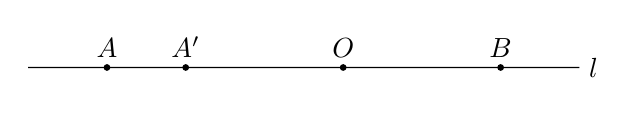
\begin{tikzpicture}
\draw[fill=black] (-3,0)--(-2,0)node[above]{\(A\)}circle(1pt)
--(-1,0)node[above]{\(A'\)}circle(1pt)
--(1,0)node[above]{\(O\)}circle(1pt)
--(3,0)node[above]{\(B\)}circle(1pt)--(4,0)node[right]{\(l\)};
\end{tikzpicture}
\caption{射线}
\label{figure:欧氏几何.射线}
\end{figure}
\end{definition}

\begin{definition}
若干条首尾相连的线段\(AB,BC,CD,\dotsc,KL\)的集合叫做一条\DefineConcept{折线段},
它连结\(A\)和\(L\)这两点.
为求简便,可将这条折线段记为\(ABCD \dotso KL\).
线段\(AB,BC,CD,\dotsc,KL\)的内点和端点都叫做这条折线段的点.
点\(A\)和点\(L\)称为“折线段的\DefineConcept{端点}”.

若折线段\(ABCD \dotso KL\)的顶点\(A,B,C,D,\dotsc,K,L\)都在同一平面上,
且它的端点\(L\)和\(A\)是同一个点,
则这条折线段就叫做一个\DefineConcept{多边形},
记为\(ABCD \dotso K\).
线段\(AB,BC,CD,\dotsc,KA\)叫做“多边形的\DefineConcept{边}”.
点\(A,B,C,D,\dotsc,K\)叫做“多边形的\DefineConcept{顶点}”.

若一个多边形有三个顶点,
则称之为\DefineConcept{三角形}.
设三角形的三个顶点分别为\(A\)、\(B\)、\(C\),
则可将其表记为以下六个符号中的任意一个:
\begin{equation*}
\begin{split}
\triangle ABC, \qquad
\triangle ACB, \qquad
\triangle BAC, \\
\triangle BCA, \qquad
\triangle CAB, \qquad
\triangle CBA.
\end{split}
\end{equation*}

若一个多边形有\(n\ (n>3)\)个顶点,
则称之为\(n\) \DefineConcept{边形}.

若一个多边形的顶点各各不同,
它的任一边内不含有顶点,
且它的任意两边无公共点,
这个多边形就叫做\DefineConcept{简单多边形}.
\end{definition}

根据\cref{theorem:欧氏几何.定理8} 可以推出下列两条推论:
\begin{theorem}\label{theorem:欧氏几何.定理9}
一平面\(\alpha\)上的每一个简单多边形,
把平面\(\alpha\)上其余点%
(即平面\(\alpha\)上的,
而不在这多边形的边上的点)%
分为\DefineConcept{内域}和\DefineConcept{外域}两个区域.
这两个区域具有如下性质:
\begin{enumerate}
	\item 若\(A\)是“内域的一个点(内点)”,
	而且\(B\)是“外域的一个点(外点)”,
	则平面\(\alpha\)上任意一条连接\(A\)和\(B\)的折线段,
	至少和多边形有一公共点.

	\item 若\(A\)和\(C\)是内点,
	而\(B\)和\(D\)是外点,
	则在平面\(\alpha\)上恒有连接\(A\)和\(C\)的折线段,
	和连接\(B\)和\(D\)的折线段,
	它们都和多边形无公共点.

	\item 平面\(\alpha\)上存在全含于外域的直线,
	而不存在全含于内域的直线.
\end{enumerate}
\end{theorem}

\begin{theorem}\label{theorem:欧氏几何.定理10}
每一平面\(\alpha\)把空间中其余点分为具有下述性质的两个区域:
\begin{enumerate}
	\item 一区域的任一点\(A\)和另一区域的任一点\(B\)所决定的线段\(AB\)内,必含有\(\alpha\)的一点.
	\item 同一区域的任意两点\(A\)和\(C\)所决定的线段\(AC\)内,恒不含有\(\alpha\)的点.
\end{enumerate}
\end{theorem}

\begin{definition}
在\cref{theorem:欧氏几何.定理10} 的条件下,
我们说“\(A\)和\(C\)这两点在空间中平面\(\alpha\)的\DefineConcept{同侧}”,
说“\(A\)和\(B\)这两点在空间中平面\(\alpha\)的\DefineConcept{异侧}”.
\end{definition}

\subsection{第三组公理:合同公理}
本组公理规定“合同”这个概念,利用它就可以规定运动的概念.

我们首先介绍角的概念.
\begin{definition}\label{definition:欧氏几何.几何元素.角}
设\(\alpha\)是任意平面,
而且\(h\)和\(k\)是\(\alpha\)上的、%
从一点\(A\)起始的、%
不属于同一直线的%
两条射线,
我们把这一对射线\(h\)和\(k\)所成的射线组叫做一个\DefineConcept{角},
记作\(\angle(h,k)\)或\(\angle(k,h)\).
称射线\(h\)和\(k\)为这个角的\DefineConcept{边}.
称点\(A\)为这个角的\DefineConcept{顶点}.

如果在\(h\)上任取一点记为\(B\),在\(k\)上任取一点记为\(C\),
那么也称角\(\angle(h,k)\)为\(\angle BAC\)或\(\angle A\).
不致混淆时,也可以用小写希腊字母表记角.

记射线\(h\)所在的直线为\(p\),射线\(k\)所在的直线为\(q\).
射线\(h\)与\(k\)(包括点\(A\))把平面\(\alpha\)上其余点分成两个区域:
在\(q\)的\(h\)侧(即\(h\)的点所在的那一侧)的,且%
在\(p\)的\(k\)侧(即\(k\)的点所在的那一侧)的区域,
叫做“角\(\angle(h,k)\)的\DefineConcept{内部}”,
或者说是在\DefineConcept{角内};
其他区域叫做“角\(\angle(h,k)\)的\DefineConcept{外部}”,
或者说是在\DefineConcept{角外}.
\end{definition}

\begin{property}
根据第一组和第二组公理,
易知任意角(不妨设为交于点\(A\)的射线\(h\)、\(k\)所成的角,即\(\angle(h,k)\))具有以下性质:
\begin{enumerate}
\item 角内、角外两个区域各含有点,连结角内两点的线段完全在角内.
\item 若点\(H\)在射线\(h\)上,点\(K\)在射线\(k\)上,则线段\(HK\)完全在角内.
\item 一条从点\(A\)起始的射线,要么完全在角内,要么完全在角外.
\item 一条完全在角内的射线与线段\(HK\)有交点.
\item 若\(B\)是一个区域的一点,而且\(C\)是另一个区域的一点,
则每一条连接\(B\)和\(C\)的折线段,要么通过点\(A\),要么与\(h\)或\(k\)至少有一个交点;
反之,若\(B\)和\(D\)是同一个区域的两点,则恒有一条连接\(B\)和\(D\)的折线段,
它既不通过点\(A\),又与\(h\)、\(k\)无交点.
\end{enumerate}
\end{property}


\begin{axiom}[合同公理]\label{axiom:欧氏几何.合同公理}
线段与线段之间、角与角之间都有一定的相互关系,我们用“合同”或“相等”这个词来描述.
\begin{enumerate}
\item 设\(A\)和\(B\)是直线\(a\)上的两点,
\(P\)是直线\(b\)上的点,
而且给定了直线\(b\)上\(P\)的一侧,
则在直线\(b\)上\(P\)的这一侧,
恒有一点\(Q\),
使得线段\(AB\)和线段\(PQ\)合同.
我们将上述关系记为\(AB \equiv PQ\).

\item 若两线段\(PQ\)和\(MN\)都和线段\(AB\)合同,
则\(PQ\)和\(MN\)也合同.

\item 设两线段\(AB\)和\(BC\)在同一直线\(a\)上,无公共点,
而且两线段\(PQ\)和\(QR\)在同一直线\(b\)上,亦无公共点.
若\(AB \equiv PQ\)且\(BC \equiv QR\),
则\(AC \equiv PR\).

\item 设给定了一个平面\(\alpha\)上的一个角\(\angle(h,k)\),
一平面\(\beta\)上的一直线\(b\),
和在\(\beta\)上\(b\)的一侧.
设\(p\)是\(b\)上的、从点\(B\)起始的一条射线,
则平面\(\beta\)上恰有一条射线\(q\),
使得\(\angle(h,k)\)与\(\angle(p,q)\)合同,
而且使得\(\angle(p,q)\)的内部在\(b\)的这给定了的一侧.
我们将上述关系记为\(\angle(h,k) \equiv \angle(p,q)\).

\item 若两个三角形\(ABC\)和\(PQR\)有下列合同式
\begin{equation*}
AB \equiv PQ, \qquad
AC \equiv PR, \qquad
\angle BAC \equiv \angle QPR,
\end{equation*}
则也恒有合同式\footnote{%
只需要交换记号,还可以同时得到另一个合同式
\(\angle ACB \equiv \angle PRQ\)
也同时成立.
}
\begin{equation*}
\angle ABC \equiv \angle PQR.
\end{equation*}
\end{enumerate}
\end{axiom}

我们在前面用点\(A\)、\(B\)所成的点组规定一条线段,并用\(AB\)或\(BA\)表示;
我们在线段的定义里,并不考虑这两点的顺序;
因此下列四个合同式的意义相同:
\begin{equation*}
AB \equiv PQ, \qquad
AB \equiv QP, \qquad
BA \equiv PR, \qquad
BA \equiv QP.
\end{equation*}

如同线段我们不考虑它的方向,在角的定义中我们也不考虑旋转方向.
因此下列四个合同式的意义也相同:
\begin{equation*}
\angle(h,k) \equiv \angle(p,q), \qquad
\angle(h,k) \equiv \angle(q,p), \qquad
\angle(k,h) \equiv \angle(p,q), \qquad
\angle(k,h) \equiv \angle(q,p).
\end{equation*}

\cref{axiom:欧氏几何.合同公理} 第3条要求线段能够相加.

\cref{axiom:欧氏几何.合同公理} 第4条可以表述为:
每一个角都能用唯一确定的方式迁移到一个给定了的平面上,
使得它沿着一条给定了的射线,并且在这射线的给定了的一侧.
藉此,我们直接保证了角的迁移的可能性与唯一性.

\cref{axiom:欧氏几何.合同公理} 第1条、第2条、第3条只论及线段的合同,
因此可以叫做“第三组公理中的直线公理”.

\cref{axiom:欧氏几何.合同公理} 第4条论及角的合同.
\cref{axiom:欧氏几何.合同公理} 第5条则把线段的合同和角的合同这两个概念联系起来.
这两条概念论及平面几何的几何元素,
因此可以叫做“第三组公理中的平面公理”.

\cref{axiom:欧氏几何.合同公理} 第1条要求线段平移的可能性,
但它还没有保证这种平移的唯一性.
只有结合\cref{axiom:欧氏几何.合同公理} 第5条,
从角的迁移的唯一性出发予以证明.
具体地,我们应用反证法,
假设把线段\(PQ\)迁移到一条从\(A\)起始的射线上可以得到不同的两点\(B\)、\(D\);
在直线\(AB\)外取一点\(C\),于是有下列合同式
\begin{equation*}
AB \equiv AD, \qquad
AC \equiv AC, \qquad
\angle BAC \equiv \angle DAC;
\end{equation*}
那么根据\cref{axiom:欧氏几何.合同公理} 第5条,得
\begin{equation*}
\angle ACB \equiv \angle ACD;
\end{equation*}
这和\cref{axiom:欧氏几何.合同公理} 第4条中要求的角的迁移的唯一性矛盾,
因此线段平移也是唯一的.

\begin{property}
线段的合同关系具有自反性、对称性和传递性,即
\begin{enumerate}
\item {\rm\bf 自反性},
\(AB \equiv AB\).

\item {\rm\bf 对称性},
\(AB \equiv PQ \implies PQ \equiv AB\)
\footnote{%
正因线段的合同关系具有对称性,
我们才能说“某两条线段互相合同”.
}.

\item {\rm\bf 传递性},
\(AB \equiv PQ \land PQ \equiv MN \implies AB \equiv MN\).
\end{enumerate}
\end{property}

\begin{property}
角的合同关系具有自反性、对称性和传递性,即
\item {\rm\bf 自反性},
\(\angle(h,k) \equiv \angle(h,k)\).

\item {\rm\bf 对称性},
\(\angle(h,k) \equiv \angle(p,q)
\implies
\angle(p,q) \equiv \angle(h,k)\).

\item {\rm\bf 传递性},
\(\angle(h,k) \equiv \angle(m,n)
\land
\angle(m,n) \equiv \angle(p,q)
\implies
\angle(h,k) \equiv \angle(p,q)\).
\end{property}
角的合同关系的自反性是显然的,
至于它的对称性、传递性和可加性,
则留待以后予以证明.

\subsection{合同公理的推论}
\begin{definition}
两角共顶点,共一边,而且不公共的两边合成一条直线的,叫做\DefineConcept{邻补角}.
\end{definition}
\begin{definition}
两角共顶点,而且它们的边合成两条直线的,叫做\DefineConcept{对顶角}.
\end{definition}
\begin{definition}
一个角和它的邻补角合同的,叫做\DefineConcept{直角}.
\end{definition}

\begin{theorem}\label{theorem:欧氏几何.定理11}
若一个三角形中的两边合同,和这两边相对的两角就也合同\footnote{%
换言之,等腰三角形的底角相等.
}.
\end{theorem}

\begin{definition}
若两个三角形\(ABC\)和\(PQR\)满足下列所有的合同式
\begin{equation*}
\begin{split}
AB \equiv PQ, \qquad
AC \equiv PR, \qquad
BC \equiv QR, \\
\angle A \equiv \angle P, \qquad
\angle B \equiv \angle Q, \qquad
\angle C \equiv \angle R,
\end{split}
\end{equation*}
就说“三角形\(ABC\)合同于三角形\(PQR\)”,
或者说“三角形\(ABC\)和三角形\(PQR\)是全等三角形”,
或者说“三角形\(ABC\)、\(PQR\)全等”,
记为\(\triangle ABC \cong \triangle PQR\).
\end{definition}

\begin{theorem}[三角形的合同定理1]\label{theorem:欧氏几何.定理12}
若两个三角形\(ABC\)、\(PQR\)有下列合同式
\begin{equation*}
AB \equiv PQ, \qquad
AC \equiv PR, \qquad
\angle A \equiv \angle P,
\end{equation*}
则\(\triangle ABC \cong \triangle PQR\).
\end{theorem}

\begin{theorem}[三角形的合同定理2]\label{theorem:欧氏几何.定理13}
若两个三角形\(ABC\)、\(PQR\)有下列合同式
\begin{equation*}
AB \equiv PQ, \qquad
\angle A \equiv \angle P,
\angle B \equiv \angle Q,
\end{equation*}
则\(\triangle ABC \cong \triangle PQR\).
\end{theorem}

\begin{theorem}\label{theorem:欧氏几何.定理14}
设\(\angle ABC\)的邻补角为\(\angle CBD\),
\(\angle PQR\)的邻补角为\(\angle RQS\).
若\(\angle ABC \equiv \angle PQR\),
则\(\angle CBD \equiv \angle RQS\).
\end{theorem}

\begin{corollary}\label{theorem:欧氏几何.对顶角合同}
任意一个角和它的对顶角合同.
\end{corollary}

\begin{corollary}\label{theorem:欧氏几何.直角存在}
直角存在.
\begin{proof}
把任意一个角迁移到沿着一条从点\(O\)起始的射线\(OA\),
而且迁移到这射线的两侧.
在新得到的这两个角的另外两条边上,
取线段\(OB \equiv OC\),
线段\(BC\)交射线\(OA\)于一点\(D\).

若点\(D\)就是点\(O\),
\(\angle BOA\)和\(\angle COA\)是合同的邻补角,所以是直角.

若点\(D\)在射线\(OA\)上,
或在与\(OA\)恰好反向的射线上,
总有\(\angle DOB \equiv \angle DOC\);
根据\cref{axiom:欧氏几何.合同公理} 第2条,
每一条线段都和它自己合同,即\(OD \equiv OD\);
再根据\cref{axiom:欧氏几何.合同公理} 第5条,
就有\(\angle ODB \equiv \angle ODC\).
\end{proof}
\end{corollary}

\begin{theorem}\label{theorem:欧氏几何.定理15}
设\(h\)、\(k\)和\(l\)是一平面\(\alpha\)上的、从一点\(M\)起始的三条射线,
而且\(p\)、\(q\)和\(r\)是一平面\(\beta\)上的、从一点\(N\)起始的三条射线;%
又设\(h\)和\(k\)分别在\(l\)的同侧(或异侧),
且\(p\)和\(q\)也分别在\(r\)的同侧(或异侧).
若
\begin{equation*}
\angle(h,l) \equiv \angle(p,r)
\quad\text{且}\quad
\angle(k,l) \equiv \angle(q,r),
\end{equation*}
则
\begin{equation*}
\angle(h,k) \equiv \angle(p,q).
\end{equation*}
\end{theorem}

\begin{theorem}\label{theorem:欧氏几何.定理16}
设平面\(\alpha\)上的\(\angle(h,k)\)合同于平面\(\beta\)上的\(\angle(p,q)\),
而且\(l\)是平面\(\alpha\)上的、从\(\angle(h,k)\)的顶点起始的、在\(\angle(h,k)\)角内的一条射线.
这时平面\(\beta\)上恒恰有一条从\(\angle(p,q)\)的顶点起始的、在\(\angle(p,q)\)角内的一条射线\(r\),
使得
\begin{equation*}
\angle(h,l) \equiv \angle(p,r), \qquad
\angle(k,l) \equiv \angle(q,r).
\end{equation*}
\end{theorem}

\begin{theorem}\label{theorem:欧氏几何.定理17}
若两点\(C\)和\(D\)在直线\(AB\)的异侧,
而且\(AC \equiv AD\)、\(BC \equiv BD\),
则\(\angle ABC \equiv \angle ABD\).
\end{theorem}

\begin{theorem}[三角形的合同定理3]\label{theorem:欧氏几何.定理18}
若两个三角形\(ABC\)和\(PQR\)的每对对应边合同,即
\begin{equation*}
AB \equiv PQ, \qquad
AC \equiv PR, \qquad
BC \equiv QR,
\end{equation*}
则\(\triangle ABC \cong \triangle PQR\).
\end{theorem}

\begin{theorem}\label{theorem:欧氏几何.定理19}
若两个角\(\angle(a,b)\)和\(\angle(c,d)\)都合同于第三个角\(\angle(e,f)\),
则\(\angle(a,b)\)也合同于\(\angle(c,d)\).
\end{theorem}
由此,我们证明了角的合同关系具有对称性、传递性.

现在我们就可以比较角的大小了.

\begin{theorem}\label{theorem:欧氏几何.定理20}
如\cref{figure:欧氏几何.图20},
给定任意两个角\(\angle(h,k)\)和\(\angle(p,r)\).
设迁移\(\angle(h,k)\)到沿着\(p\),而且在\(p\)的\(r\)侧时,所得到的射线是\(q\);
又迁移\(\angle(p,r)\)到沿着\(h\),而且在\(h\)的\(k\)侧时,所得到的射线是\(l\);
这时,若\(q\)在\(\angle(p,r)\)内,则\(l\)在\(\angle(h,k)\)外.
反之也成立.
\end{theorem}

\begin{figure}[htb]
	\centering
	\begin{tikzpicture}
		\pgfmathsetmacro{\r}{3}
		\begin{scope}
			\draw(0,0)--(\r,0)node[right]{\(h\)};
			\pgfmathsetmacro{\kx}{\r*cos(45)}
			\pgfmathsetmacro{\ky}{\r*sin(45)}
			\draw(0,0)--(\kx,\ky)node[right]{\(k\)};
			\pgfmathsetmacro{\lx}{\r*cos(60)}
			\pgfmathsetmacro{\ly}{\r*sin(60)}
			\draw(0,0)--(\lx,\ly)node[above]{\(l\)};
		\end{scope}
		\begin{scope}[xshift=6cm]
			\draw(0,0)--(\r,0)node[right]{\(p\)};
			\pgfmathsetmacro{\kx}{\r*cos(45)}
			\pgfmathsetmacro{\ky}{\r*sin(45)}
			\draw(0,0)--(\kx,\ky)node[right]{\(q\)};
			\pgfmathsetmacro{\lx}{\r*cos(60)}
			\pgfmathsetmacro{\ly}{\r*sin(60)}
			\draw(0,0)--(\lx,\ly)node[above]{\(r\)};
		\end{scope}
	\end{tikzpicture}
	\caption{}
	\label{figure:欧氏几何.图20}
\end{figure}

\begin{definition}
在\cref{theorem:欧氏几何.定理20} 中,
若\(q\)在\(\angle(p,r)\)内,则称“\(\angle(h,k)\)小于\(\angle(p,r)\)”,记为\(\angle(h,k) < \angle(p,r)\).
若\(q\)在\(\angle(p,r)\)外,则称“\(\angle(h,k)\)大于\(\angle(p,r)\)”,记为\(\angle(h,k) > \angle(p,r)\).
\end{definition}

因此,两个角\(\alpha,\beta\)恒恰适合以下三种情形之一:
\begin{itemize}
	\item \(\alpha<\beta\)和\(\beta>\alpha\).
	\item \(\alpha\equiv\beta\).
	\item \(\alpha>\beta\)和\(\beta<\alpha\).
\end{itemize}

角的大小的比较有传递性.
若有下列三种情形
\begin{itemize}
	\item \(\alpha>\beta,\beta>\gamma\),
	\item \(\alpha>\beta,\beta\equiv\gamma\),
	\item \(\alpha\equiv\beta,\beta>\gamma\),
\end{itemize}
之一,则\begin{equation*}
	\alpha>\gamma.
\end{equation*}

\begin{theorem}\label{theorem:欧氏几何.定理21}
所有的直角都互相合同.
\end{theorem}

\begin{definition}
一个角大于它的邻补角的,也就是大于一直角的,叫做\DefineConcept{钝角};
小于它的邻补角的,也就是小于一直角的,叫做\DefineConcept{锐角}.
\end{definition}

\begin{definition}
\(\triangle ABC\)的\(\angle ABC\)、\(\angle BCA\)和\(\angle CAB\)
叫做这个三角形的\DefineConcept{内角},简称为这个三角形的\DefineConcept{角};
它们的邻补角叫做这个三角形的\DefineConcept{外角}.
\end{definition}

\begin{theorem}[外角定理]\label{theorem:欧氏几何.定理22}
在三角形中,一个外角大于其任一不相邻的内角.
\end{theorem}

下列定理是外角定理的重要推论.

\begin{theorem}\label{theorem:欧氏几何.定理23}
在三角形中,长边所对的角大于短边所对的角.
\end{theorem}

\begin{theorem}\label{theorem:欧氏几何.定理24}
若三角形有两角合同,则有两边合同.
\end{theorem}
这是\cref{theorem:欧氏几何.定理11} 的逆定理,
也是\cref{theorem:欧氏几何.定理23} 的直接推论.

从\cref{theorem:欧氏几何.定理22},
还能很简单地证得下述对三角形的合同定理二的补充.
\begin{theorem}\label{theorem:欧氏几何.定理25}
若\(\triangle ABC\)和\(\triangle DEF\)有下列合同式\begin{equation*}
	AB \equiv DE, \qquad
	\angle A \equiv \angle D, \qquad
	\angle C \equiv \angle F,
\end{equation*}
则这两个三角形合同.
\end{theorem}

\begin{theorem}\label{theorem:欧氏几何.定理26}
每一线段都能二等分.
\end{theorem}

类似地,从\cref{theorem:欧氏几何.定理11} 和\cref{theorem:欧氏几何.定理26},能直接推证下列事实:
\begin{theorem}
每一角都能二等分.
\end{theorem}

合同的概念可以推广应用到任意的图形上去.

\begin{definition}
设\(A,B,C,D,\dotsc,K,L\)是直线\(\alpha\)上的一个点列,
\(A',B',C',D',\dotsc,K',L'\)是直线\(\alpha'\)上的一个点列,
而且所有的对应线段都两两合同,
那么称这两个点列互相合同.
\(A\)和\(A'\)、\(B\)和\(B'\),一直到\(L\)和\(L'\),叫做这\emph{合同点列}的对应点.
\end{definition}

\begin{theorem}\label{theorem:欧氏几何.定理27}
两个合同的点列的点的顺序相同.
\end{theorem}

\begin{definition}
任意有限个点叫做一个\DefineConcept{图形}.
一个图形的点,若都在一个平面上,这图形就叫做一个\DefineConcept{平面图形}.
\end{definition}

两个图形的点之间若有一个一一对应的关系,
使得由此规定的每对对应的线段都互相合同,
且每对对应的角都互相合同,
那么这两个图形合同.

由\cref{theorem:欧氏几何.定理14}
和\cref{theorem:欧氏几何.定理27},
可知合同图形有下述性质:
若一个图形中的三个点在一条直线上,
则每一个和它合同图形中的对应的三个点也在一条直线上.
合同图形中的、对应平面上的对应点,
对于对应直线而言的顺序相同;
对应直线上的对应点顺序也相同.

平面的和空间的最普遍的合同定理如下:
\begin{theorem}\label{theorem:欧氏几何.定理28}
设\((A,B,C,\dotsc,L)\)
和\((A',B',C',\dotsc,L')\)
是两个合同的平面图形.
若\(P\)是第一个图形的平面上的一点,
则第二个图形的平面上恒有一点\(P'\)存在,
使得\((A,B,C,\dotsc,L,P)\)
和\((A',B',C',\dotsc,L',P')\)还是合同的图形.
若\((A,B,C,\dotsc,L)\)至少含有不在同一条直线上的三点,
则\(P'\)只有一个可能的作法.
\end{theorem}

\begin{theorem}\label{theorem:欧氏几何.定理29}
设\((A,B,C,\dotsc,L)\)
和\((A',B',C',\dotsc,L')\)
是两个合同的图形.
若\(P\)是任意一点,
则恒有一点\(P'\)存在,
使得\((A,B,C,\dotsc,L,P)\)
和\((A',B',C',\dotsc,L',P')\)还是合同的图形.
若\((A,B,C,\dotsc,L)\)至少含有不在同一平面上的四点,
则\(P'\)只有一个可能的作法.
\end{theorem}

\cref{theorem:欧氏几何.定理29} 说出了所有关于合同的空间事实,
因此,空间中运动的性质,都是上述的直线的和平面的五条合同公理(结合着第一组和第二组公理)的推论.

\subsection{第四组公理:平行公理}
设\(\alpha\)是任一平面,
\(a\)是\(\alpha\)上的任一直线,
而且\(A\)是\(\alpha\)上的、但不在\(a\)上的一点,
在\(\alpha\)上作一直线\(c\),
通过\(A\)且和\(a\)相交,
再在\(\alpha\)上作一直线\(b\),通过\(A\),
且使得\(c\)交\(a\)和\(b\)于相等的同位角.
从\hyperref[theorem:欧氏几何.定理22]{外角定理},
易知\(a\)和\(b\)这两直线无公共点,这就是说,
在一平面\(\alpha\)上,而且通过一直线\(a\)外的一点\(A\),
恒有一直线不和\(a\)相交.

现在可将平行公理叙述如下:
\begin{axiom}[平行公理、欧几里得公理]\label{axiom:欧氏几何.平行公理}
设\(a\)是任一直线,\(A\)是\(a\)外的任一点.
在\(a\)和\(A\)所决定的平面上,
至多有一条直线通过\(A\),而且不和\(a\)相交.
\end{axiom}

根据上文和平行公理,我们知道:
在\(a\)和\(A\)所决定的平面上,恰有一直线,通过\(A\)且不和\(a\)相交,
我们把这条直线叫做“通过\(A\)的\(a\)的\DefineConcept{平行直线}”.

平行公理和下述的要求等价:
如果一平面上的\(a\)和\(b\)两直线都不和这平面上的第三条直线\(c\)相交,
那么\(a\)和\(b\)也不相交.

事实上,如果\(a\)和\(b\)有一公共点\(A\),那么在同一平面上,
就有了\(a\)和\(b\)这两条直线,都通过\(A\)而且不和\(c\)相交.
这和平行公理矛盾.
反之,从上述要求,也易推得平行公理.

平行公理是一条平面公理.
它的引入,使得几何的基础大大地简单化了,也使得几何的构造容易得多了.

例如,在合同公理之外,再加上平行公理,不难得到下列熟知的事实:
\begin{theorem}\label{theorem:欧氏几何.定理30}
若两平行直线被第三条直线所截,则同位角合同,内错角也合同;
反之,若同位角合同,或内错角合同,则前两直线平行.
\end{theorem}

\begin{theorem}\label{theorem:欧氏几何.定理31}
三角形的三个内角的和等于两个直角的和.
\end{theorem}
\begin{figure}[htb]
	\centering
	\begin{tikzpicture}
		\coordinate (A) at (0,0);
		\coordinate (B) at (4,0);
		\coordinate (C) at (3,2);
		\coordinate (P) at (2,2);
		\coordinate (Q) at (4,2);
		\draw (A)node[left]{\(A\)}
				-- (B)node[right]{\(B\)}
				-- (C)node[above]{\(C\)} -- (A);
		\draw (P)node[left]{\(P\)} -- (Q)node[right]{\(Q\)};
		\draw pic[draw=blue,angle radius=5mm]{angle=B--A--C}
				pic[draw=blue,angle radius=6mm]{angle=B--A--C}
				pic[draw=blue,angle radius=5mm]{angle=P--C--A}
				pic[draw=blue,angle radius=6mm]{angle=P--C--A}
				pic[draw=orange,angle radius=4mm]{angle=C--B--A}
				pic[draw=orange,angle radius=4mm]{angle=B--C--Q};
	\end{tikzpicture}
	\caption{}
	\label{figure:欧氏几何.三角形内角和等于平角}
\end{figure}

\begin{definition}
设\(M\)是一平面\(\alpha\)上的任一点.
考虑\(\alpha\)上的所有的那些点\(A\),
它们使线段\(MA\)都互相合同的.
这种点\(A\)的全体叫做一个\DefineConcept{圆},
点\(M\)叫做“这个圆的\DefineConcept{中心}”,简称\DefineConcept{圆心}.
\end{definition}

根据这个定义,我们容易从第三组和第四组公理,推证关于圆的若干熟知的定理.
特别是下述的定理:
通过不在同一条直线上的三点,能作一圆;
关于同一条弦上的圆周角合同的定理;
关于内接于圆的一个四边形的角的定理.

\subsection{第五组公理:连续公理}

\begin{axiom}[连续公理]
关于线段、角的度量,有如下公理:
\begin{enumerate}
	\item (度量公理,阿基米德公理).
	若\(AB\)和\(CD\)是任意两线段,则必存在一个数\(n\)使得沿\(A\)到\(B\)的射线上,
	自\(A\)作首尾相接的\(n\)个线段\(CD\),必将越过\(B\)点.
	\item (直线完备公理).
	一直线上的点集联通其顺序关系与合同关系不可能再这样扩充,
	使得这直线上原来元素之间所具有的关系,
	从第一组、第二组、第三组公理所推出的直线顺序与合同的基本性质\footnote{%
	所谓“基本性质”是指第二组第一至三条公理和\cref{theorem:欧氏几何.定理5} 中所叙述的顺序性质,
	以及第三组第一至第三条公理中所叙述的合同性质连同迁移线段的唯一性.}
	以及度量公理都仍旧保持\footnote{%
	所谓“仍旧保持”是指,当点集扩充后,顺序关系及合同关系也将延续到扩充后的点集中去.
	我们注意到第一组第三条公理在各种扩充后,不言而喻地仍然保持,
	至于在所考虑的扩充下,\cref{theorem:欧氏几何.定理3} 仍能成立,
	则是保持阿基米德公理的结果.}.
\end{enumerate}
\end{axiom}

完备公理中所要求保持的诸公理之一是阿基米德公理,
这时完备公理从本质上能以建立所不可缺少的一个条件.
其实我们能够证明:
若直线上的一个点集能满足上面所列举的关于顺序公理和定理以及合同公理和定理,
这点集就恒能够增加新点,使扩充后的点集还满足这里所提到的诸公理;
也就是说,如果一条完备公理,只要求保持这里所提到的诸公理和定理,
但不要求保持阿基米德公理或一条等价的公理,就要产生矛盾.

这两条连续公理都是直线公理.

下面所述更普遍的定理,主要根据直线完备公理.
\begin{theorem}[完备定理]\label{theorem:欧氏几何.定理32}
几何元素(即点、直线、平面)形成一个集合,
它在保持关联公理、顺序公理、合同公理和阿基米德公理,
从而更不用说,在保持全体公理的条件之下,
不可能经由点、直线和平面再行扩充.
\end{theorem}

完备定理还能表成较强的形式.
也就是在完备定理内缩要求保持的诸公理中,有些并不是绝对需要的,为了定理能够成立,
重要的倒是在所要求保持的诸公理中包含有第一组第七条公理.
其实我们能证明:
对于满足第一至第第五组公理的元素集合,恒能给添加新的点、直线和平面,
使得扩充后的心机和能满足除去第一组第七条公理之外的全体公理;
这就是说,一条完备定理若不包含第一组第七条公理或一条等价的公理,就将引出矛盾.

完备公理不是阿基米德公理的一个推论.
实际上,只有阿基米德公理,连同第一至第四组公理,
并不足以证明我们的几何和通常的笛卡尔解析几何完全相同.
但是加上了完备公理(虽然这条公理并没有直接提到收敛的概念),
就能证明(相当于戴德金分割的)确界的存在,
和关于聚点存在的波尔查诺定理,
从而才证明欧氏几何和笛卡尔几何相同.

从上文可见,连续的要求,在本质上,分成两个不同的部分:
阿基米德公理和完备公理;
前者的作用是替连续的要求做准备,
后者为完成整个公理系统作基础.

在本章后面的研究中,我们主要只用阿基米德公理作根据,而普遍地不假设完备公理.

\section{平面三角形}

\begin{theorem}
三角形内角和为\(\pi\).
\begin{proof}
设有\(\triangle ABC\).
过点\(C\)作平行于线段\(AB\)的直线\(PQ\).

由内错角相等,有\begin{equation*}
\angle{PCA} = \angle{CAB}, \quad \angle{QCB} = \angle{CBA},
\end{equation*}又由\(\angle{PCA}+\angle{ACB}+\angle{QCB}=\pi\),可得\begin{equation*}
\angle{CAB}+\angle{ACB}+\angle{QCB}=\pi.
\qedhere
\end{equation*}
\end{proof}
\end{theorem}

\begin{theorem}[正弦定理]
设任意三角形\(\triangle ABC\)的外接圆半径为\(R\),则\begin{equation}
\frac{a}{\sin A}
= \frac{b}{\sin B}
= \frac{c}{\sin C}
= 2R.
\end{equation}
\end{theorem}

\begin{theorem}[余弦定理]
设任意三角形\(\triangle ABC\),有\begin{equation}
c^2 = a^2 + b^2 - 2ab \cos C.
\end{equation}
\end{theorem}
可以看出,勾股定理是余弦定理的特殊情况,即当\(C = \frac{\pi}{2}\)时,有\(\cos C=0\),于是\(c^2 = a^2 + b^2\).

\begin{theorem}[摩尔外德公式]
%@see: https://arxiv.org/pdf/1808.08049.pdf
设任意三角形\(\triangle ABC\),则\begin{gather}
	\frac{a+b}{c}
	= \frac{\cos[(A-B)/2]}{\sin(C/2)}, \\
	\frac{a-b}{c}
	= \frac{\sin[(A-B)/2]}{\cos(C/2)}.
\end{gather}
\end{theorem}

\begin{theorem}[正切定理]
设任意三角形\(\triangle ABC\),有\begin{equation}
\frac{a-b}{a+b} = \frac{\tan[(A-B)/2]}{\tan[(A+B)/2]}.
\end{equation}
\end{theorem}

\section{圆}
\subsection{圆的概念}
\subsection{圆的性质}
\subsection{圆的周长\ 圆周率}
\begin{definition}
定义:圆的周长\(C\)与其直径\(2R\)之比称为\DefineConcept{圆周率},记作\(\pi\),即\begin{equation*}
\pi = \frac{C}{2R}.
\end{equation*}
\end{definition}
由于圆周率是一个常数,那么已知圆的直径(或半径)可以求得圆的周长,而已知圆的周长可以求得圆的直径(或半径).

\begin{property}
给定圆上任意一段弧,若它的角度为\(\theta\),那么弧长为\(\theta r\).
\end{property}

\begin{corollary}
如下图,在单位圆上,当圆弧的角度\(\theta\)为锐角,即\(0<\theta<\pi/2\)时,\(\theta > x\). \begin{center}
\begin{tikzpicture}[scale=4]
%\draw[help lines, color=gray!30, dashed] (0,0) grid (1,1);
\pgfmathsetmacro{\u}{sqrt(3)/2}
\coordinate (O) at (0,0);
\coordinate (A) at (\u,0);
\coordinate (B) at (\u,1/2);
\draw (1,0)arc[start angle=0,end angle=30,radius=1]node[midway,right]{\(\theta\)} -- (0,0)node[midway,above left]{\(1\)} -- (1,0)
	(A) -- (B)node[midway,left]{\(x\)};
\draw pic["\(\theta\)",draw=orange,-,angle eccentricity=1.7,angle radius=5mm]{angle=A--O--B} pic[draw=gray,-,angle radius=0.3cm]{right angle=B--A--O};
\end{tikzpicture}
\end{center}
\end{corollary}

\section{平面凸多边形}
\begin{theorem}
设凸多边形的边数为\(n\),则其内角和为\((n-2)\pi\).
\end{theorem}
如图,在凸多边形内部任取一点\(P\),连接该点与凸多边形各顶点,可以得到\(n\)个三角形.
因为三角形内角和为\(\pi\),所以\(n\)个三角形内角和的总和为\(n\pi\),
再减去各三角形\(\angle P\)之和\(2\pi\),可知凸\(n\)边形的内角和为\((n-2)\pi\).
\begin{figure}[htb]
	\centering
	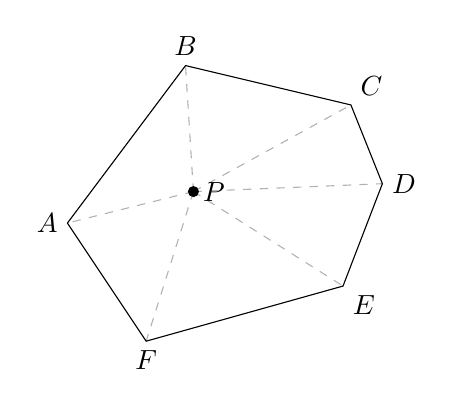
\begin{tikzpicture}
		\coordinate (A1) at (0,2);
		\coordinate (A2) at (1.5,4);
		\coordinate (A3) at (3.6,3.5);
		\coordinate (A4) at (4,2.5);
		\coordinate (A5) at (3.5,1.2);
		\coordinate (A6) at (1,0.5);
		\coordinate (P) at (1.6,2.4);
		\draw[dashed,color=black!30] (P)--(A1) (P)--(A2)
			(P)--(A3) (P)--(A4) (P)--(A5) (P)--(A6);
		\draw (A1)node[left]{\(A\)}--(A2)node[above]{\(B\)}
			--(A3)node[above right]{\(C\)}
			--(A4)node[right]{\(D\)}
			--(A5)node[below right]{\(E\)}
			--(A6)node[below]{\(F\)}--(A1)
			(P)node[right]{\(P\)};
		\fill (P)circle(2pt);
	\end{tikzpicture}
	\caption{}
\end{figure}

\begin{theorem}
凸多边形的外角和为\(2\pi\).
\end{theorem}

\section{凸多面体}
\begin{theorem}[欧拉公式]
设凸多面体的顶点数、棱数、面数分别为\(V\)、\(E\)、\(F\),则有\begin{equation*}
	V - E + F = 2.
\end{equation*}
\end{theorem}

\begin{definition}
\DefineConcept{正凸多面体}(简称\DefineConcept{正多面体}),
是指满足以下条件的凸多面体:
\begin{enumerate}
	\item 正多面体的面由正多边形构成;
	\item 正多面体的各个顶角相等;
	\item 正多面体的各条棱长相等.
\end{enumerate}
\end{definition}

\begin{corollary}
正凸多面体只有5种:三四面体、正方体、正八面体、正十二面体、正二十面体.
\end{corollary}
